\documentclass[12pt]{article}

\usepackage{graphicx}
\usepackage{float}
\usepackage{subcaption}
\usepackage{amsfonts}
\usepackage{amsmath}
\usepackage{amssymb}

\title{Progress Report: Parallel Controllable Texture Synthesis}
\author{Matthew McMullan and Ian Ooi}
\date{December 4, 2012}

\begin{document}
    \maketitle
    \section{Current Progress}
        So far, we have implemented upsampling and jitter, the first two steps of the general algorithm.  Our upsampling implementation uses a fragment shader which renders a series of textures to produce and image pyramid.  The fragment shader produces the different sizes of images by starting at a 1 by 1 pixel texture of coordinates (where the coordinates correspond to coordinates in the exemplar).  Every round, the number of pixels quadruples, with each pixel creating an extra pixel to the right, below it, and diagonally to the right and below.  The pixels of the image are shifted to accomodate the extra pixels, and the new pixels are filled with the pixel coordinates from the exemplar.
        
      Jitter is accomplished through the use of a simplex noise implementation. We modify the destination locations in each level of the image pyramid with deterministcally calculated pseudo-random noise, with each pixel of the result storing the pixel coordinates of a texel in the exemplar.  We choose a direction to shift the pixel, either $+1$ or $-1$ based on a randomness threshold ratio $r$ individually for the x and y directions.  In order to have higher values of $r$ correspond to more randomness, the comparison is made between the generated noise value $\vec{n} \in \mathbb{R}^2$ and $\left(1 - r \right)$ where $n_i > (1-r)$ corresponds to a $+1$ and $n_i < -(1-r)$ corresponds to $-1$, with any other value resulting in no movement.  The position of the pixel-coordinate texel is then moved accordingly.  Throughout upsampling and jitter, we only work with pixel coordinates, not the actual values of the exemplar.

    \section{Results}
        \begin{figure}[H]
            \centering
            %\begin{subfigure}[h]
            %    \centering
            %    %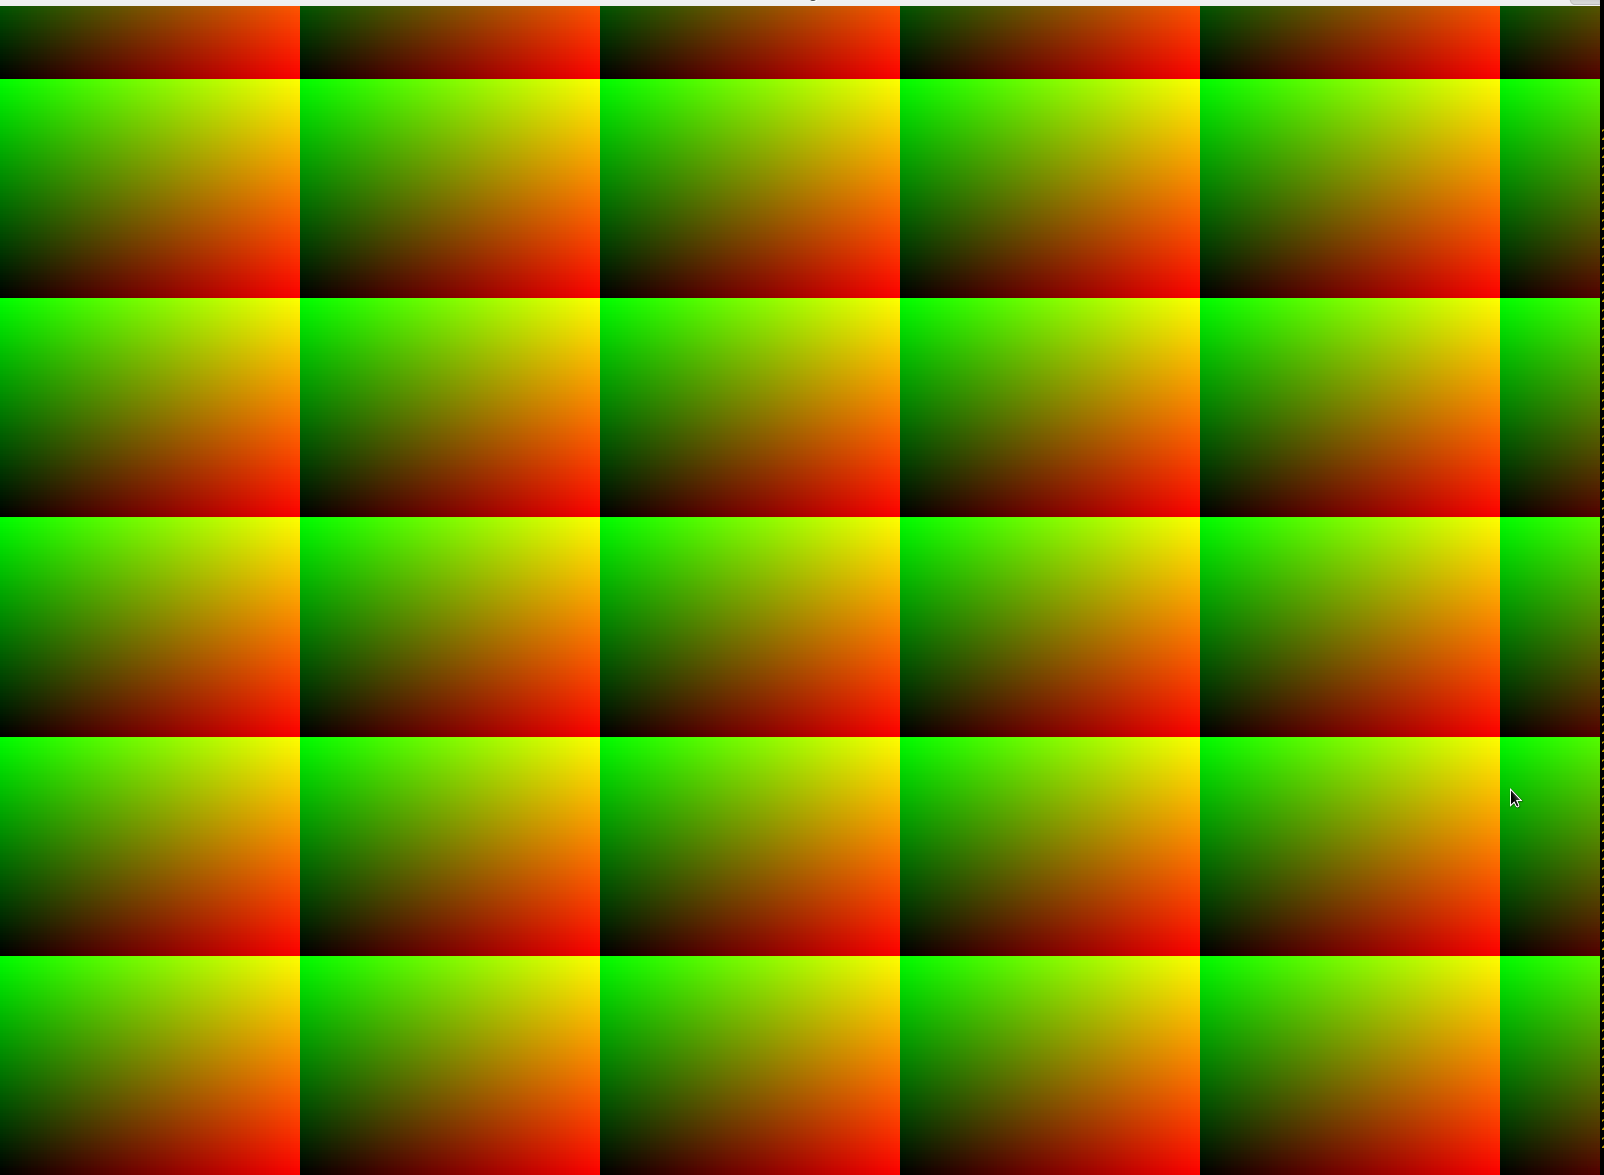
\includegraphics{result3.png}
            %    \caption{}
            %    \label{fig:grad}
            %\end{subfigure}
            \begin{subfigure}
                \centering
                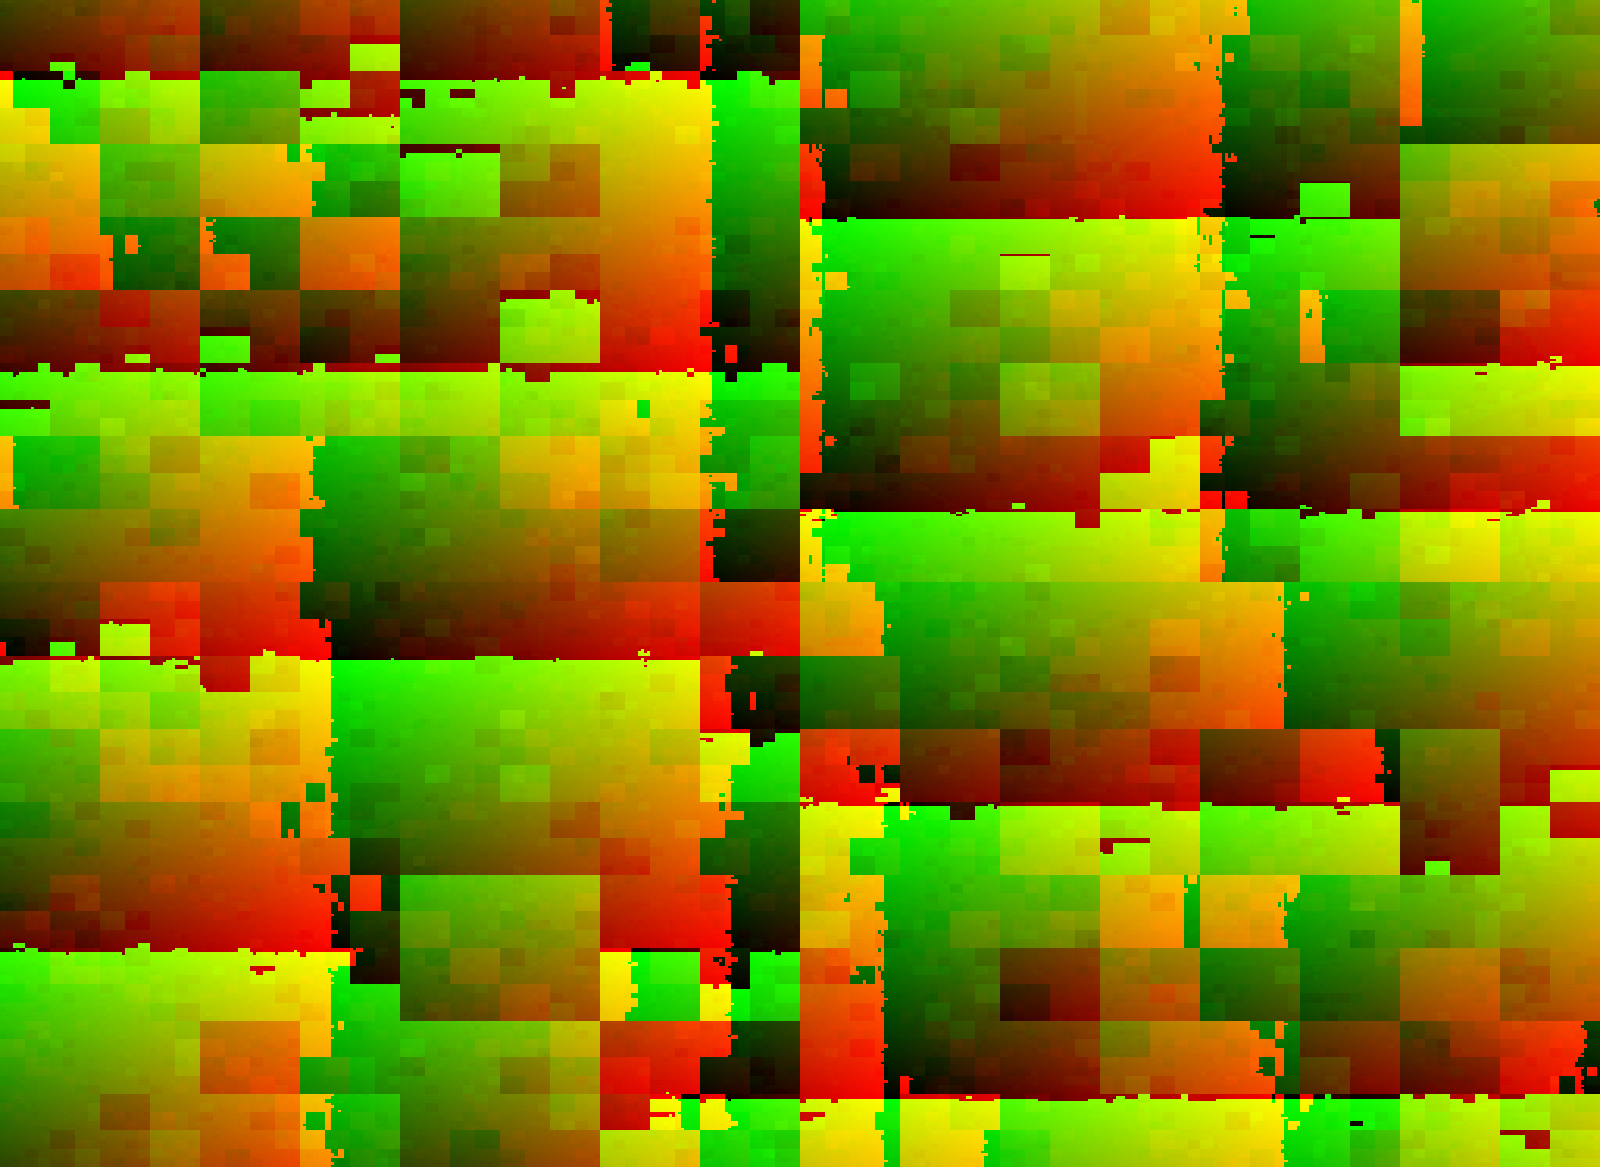
\includegraphics[width=3in]{result0.png}
                \caption{}
                \label{fig:visual}
            \end{subfigure}
            \begin{subfigure}
                \centering
                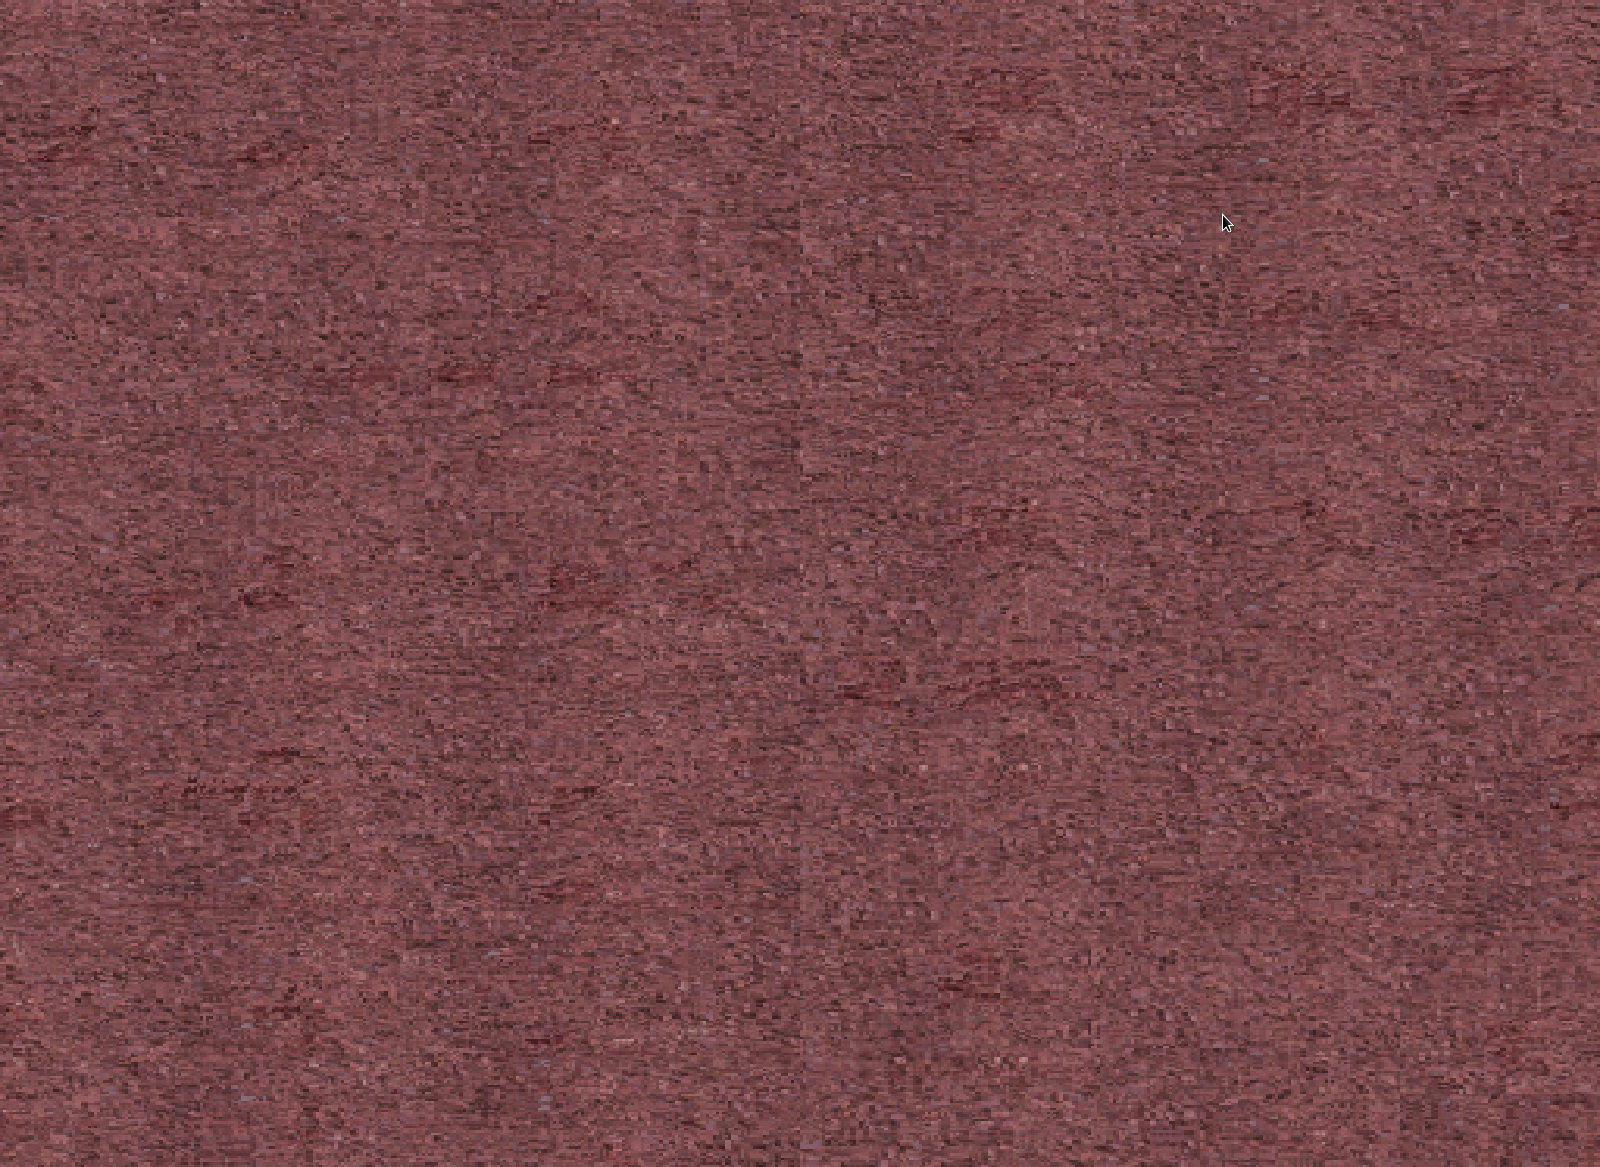
\includegraphics[width=3in]{result1.png}
                \caption{}
                \label{fig:stoch}
            \end{subfigure}
            \begin{subfigure}
                \centering
                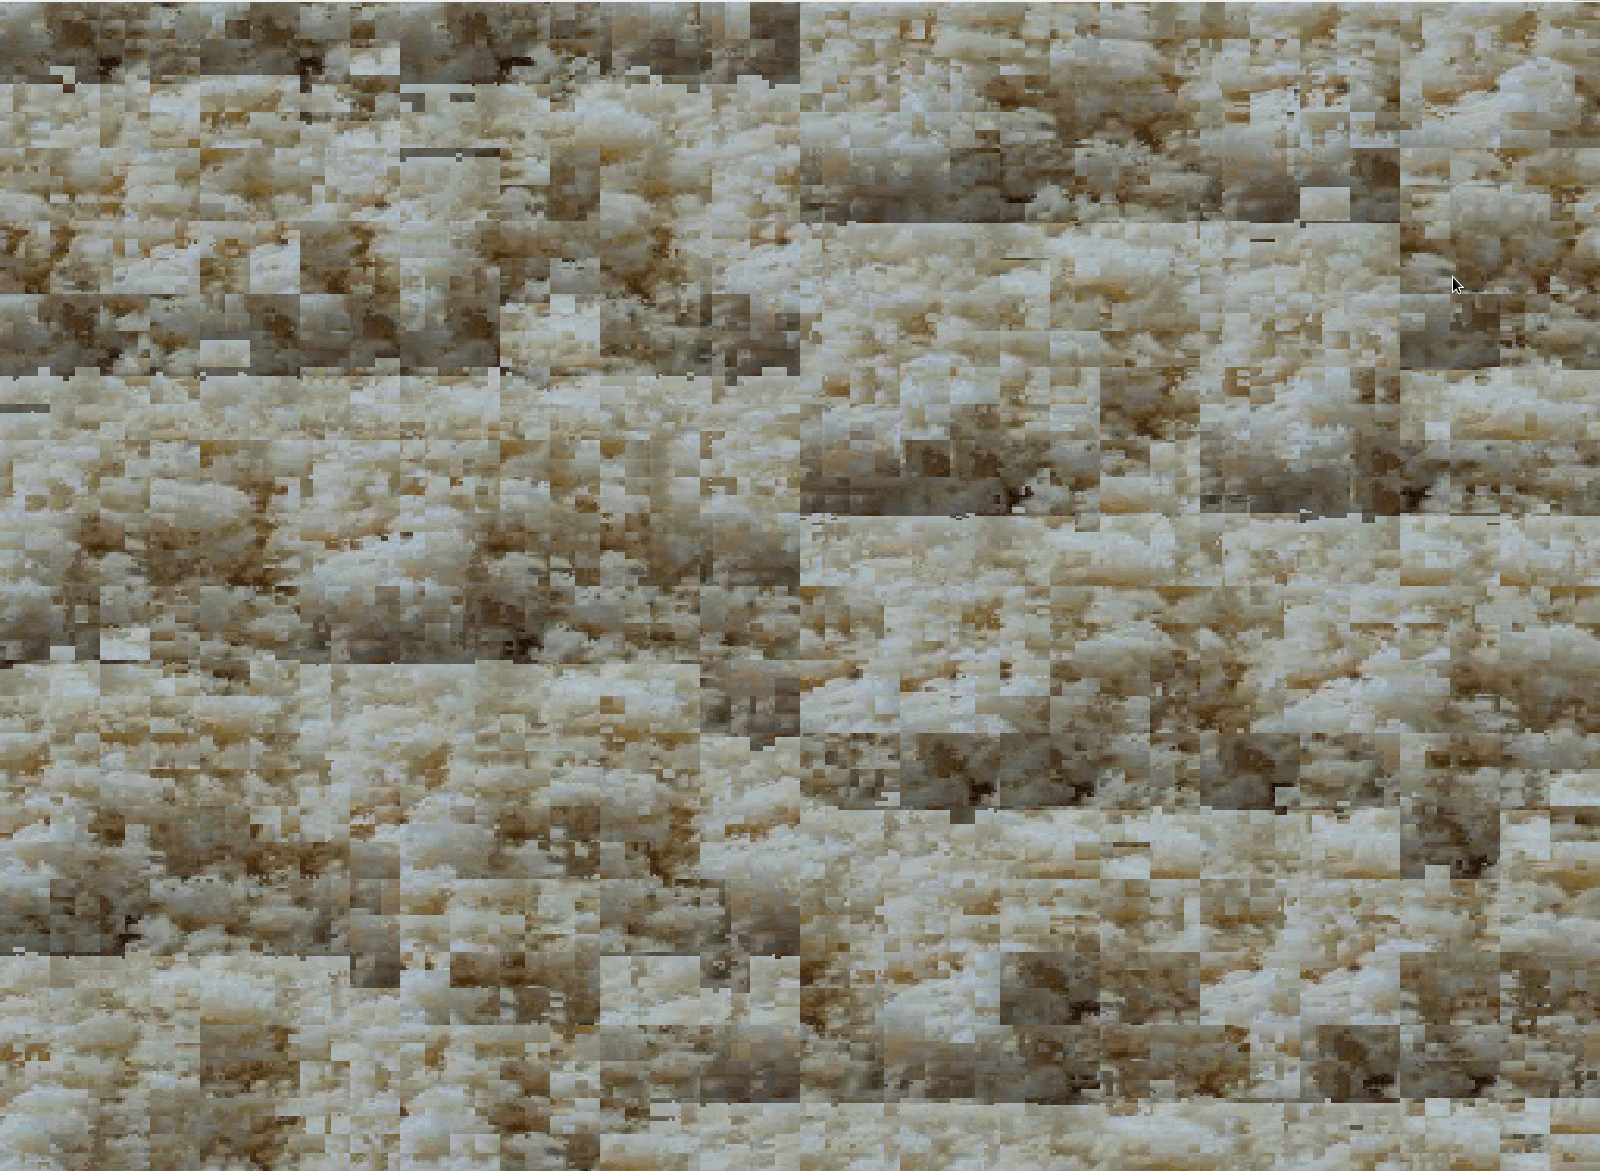
\includegraphics[width=3in]{result2.png}
                \caption{}
                \label{fig:toroid}
            \end{subfigure}
            \caption{In (\ref{fig:visual}) we show a visualization of our upscaling and jitter on a gradient, seen in} %\ref{fig:grad}
        \end{figure}
\end{document}
